% Template for PLoS
% Version 1.0 January 2009
%
% To compile to pdf, run:
% latex plos.template
% bibtex plos.template
% latex plos.template
% latex plos.template
% dvipdf plos.template

\documentclass[10pt]{article}

% amsmath package, useful for mathematical formulas
\usepackage{amsmath}
% amssymb package, useful for mathematical symbols
\usepackage{amssymb}

% graphicx package, useful for including eps and pdf graphics
% include graphics with the command \includegraphics
\usepackage{graphicx}

% cite package, to clean up citations in the main text. Do not remove.
\usepackage{cite}

\usepackage{color} 

% Use doublespacing - comment out for single spacing
%\usepackage{setspace} 
%\doublespacing


% Text layout
\topmargin 0.0cm
\oddsidemargin 0.5cm
\evensidemargin 0.5cm
\textwidth 16cm 
\textheight 21cm

% Bold the 'Figure #' in the caption and separate it with a period
% Captions will be left justified
\usepackage[labelfont=bf,labelsep=period,justification=raggedright]{caption}

% Use the PLoS provided bibtex style
\bibliographystyle{plos2009}

% Remove brackets from numbering in List of References
\makeatletter
\renewcommand{\@biblabel}[1]{\quad#1.}
\makeatother


% Leave date blank
\date{}

\pagestyle{myheadings}
%% ** EDIT HERE **


%% ** EDIT HERE **
%% PLEASE INCLUDE ALL MACROS BELOW

%% END MACROS SECTION

\begin{document}

% Title must be 150 characters or less
\begin{flushleft}
{\Large
\textbf{Supplementary Data}
}
% Insert Author names, affiliations and corresponding author email.
%\\
%Author1$^{1}$, 
%Author2$^{2}$, 
%Author3$^{3,\ast}$
%\\
%\bf{1} Author1 Dept/Program/Center, Institution Name, City, State, Country
%\\
%\bf{2} Author2 Dept/Program/Center, Institution Name, City, State, Country
%\\
%\bf{3} Author3 Dept/Program/Center, Institution Name, City, State, Country
%\\
%$\ast$ E-mail: Corresponding author@institute.edu
\end{flushleft}

% Please keep the abstract between 250 and 300 words
%\section*{Abstract}

% Please keep the Author Summary between 150 and 200 words
% Use first person. PLoS ONE authors please skip this step. 
% Author Summary not valid for PLoS ONE submissions.   
%\section*{Author Summary}

%\section*{Introduction}

% Results and Discussion can be combined.
%\section*{Results}

%\subsection*{Subsection 1}

%\subsection*{Subsection 2}

%\section*{Discussion}

% You may title this section "Methods" or "Models". 
% "Models" is not a valid title for PLoS ONE authors. However, PLoS ONE
% authors may use "Analysis" 
%\section*{Materials and Methods}

% Do NOT remove this, even if you are not including acknowledgments
%\section*{Acknowledgments}


%\section*{References}
% The bibtex filename
%\bibliography{template}

\section*{Figure Legends}
\begin{figure}[!ht]
\begin{center}
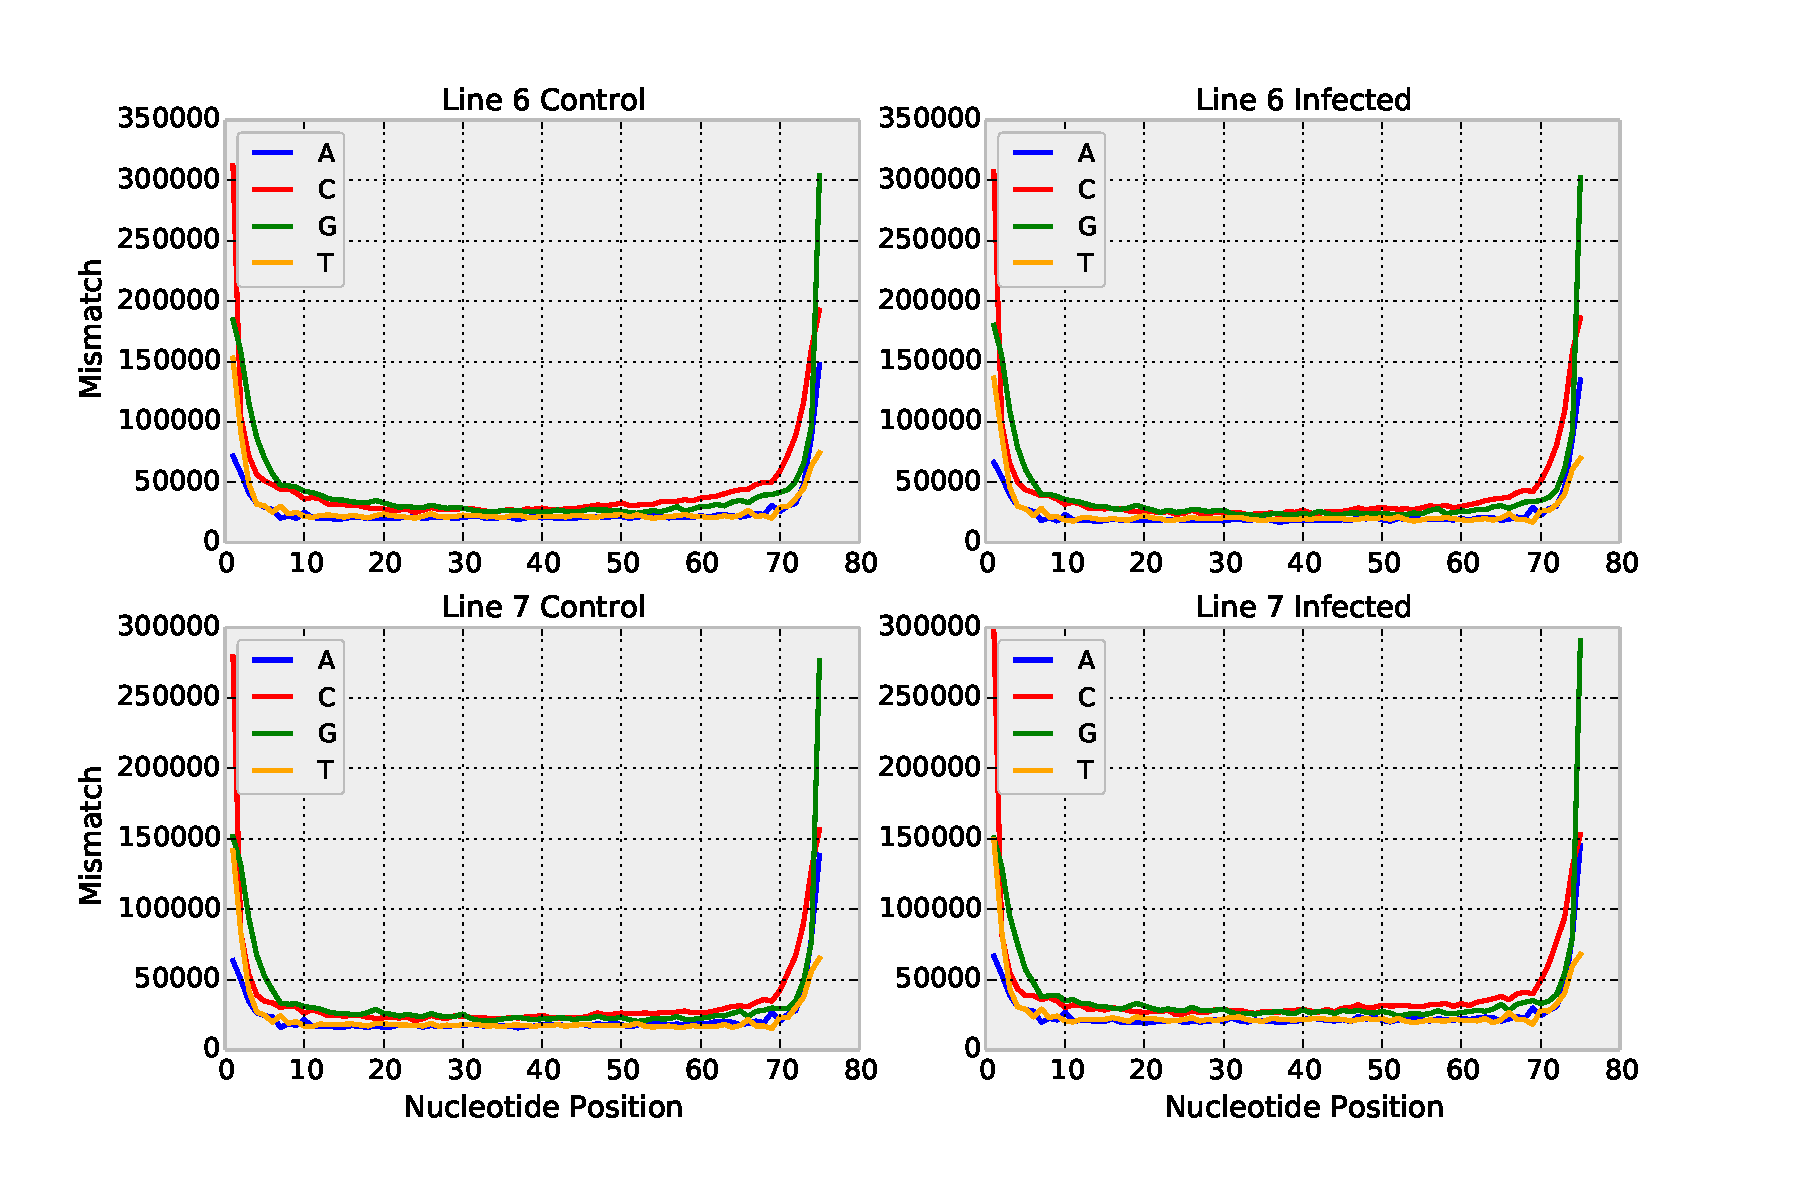
\includegraphics[width=6in]{error_profile.pdf}
\end{center}
\caption{
{\bf Mismatch profiles.} More mismatches are found in the first ten and the
last five positions of a read than other positions suggesting errors in base
calling toward both ends.}
\label{Figure_label}
\end{figure}

\begin{figure}[!ht]
\begin{center}
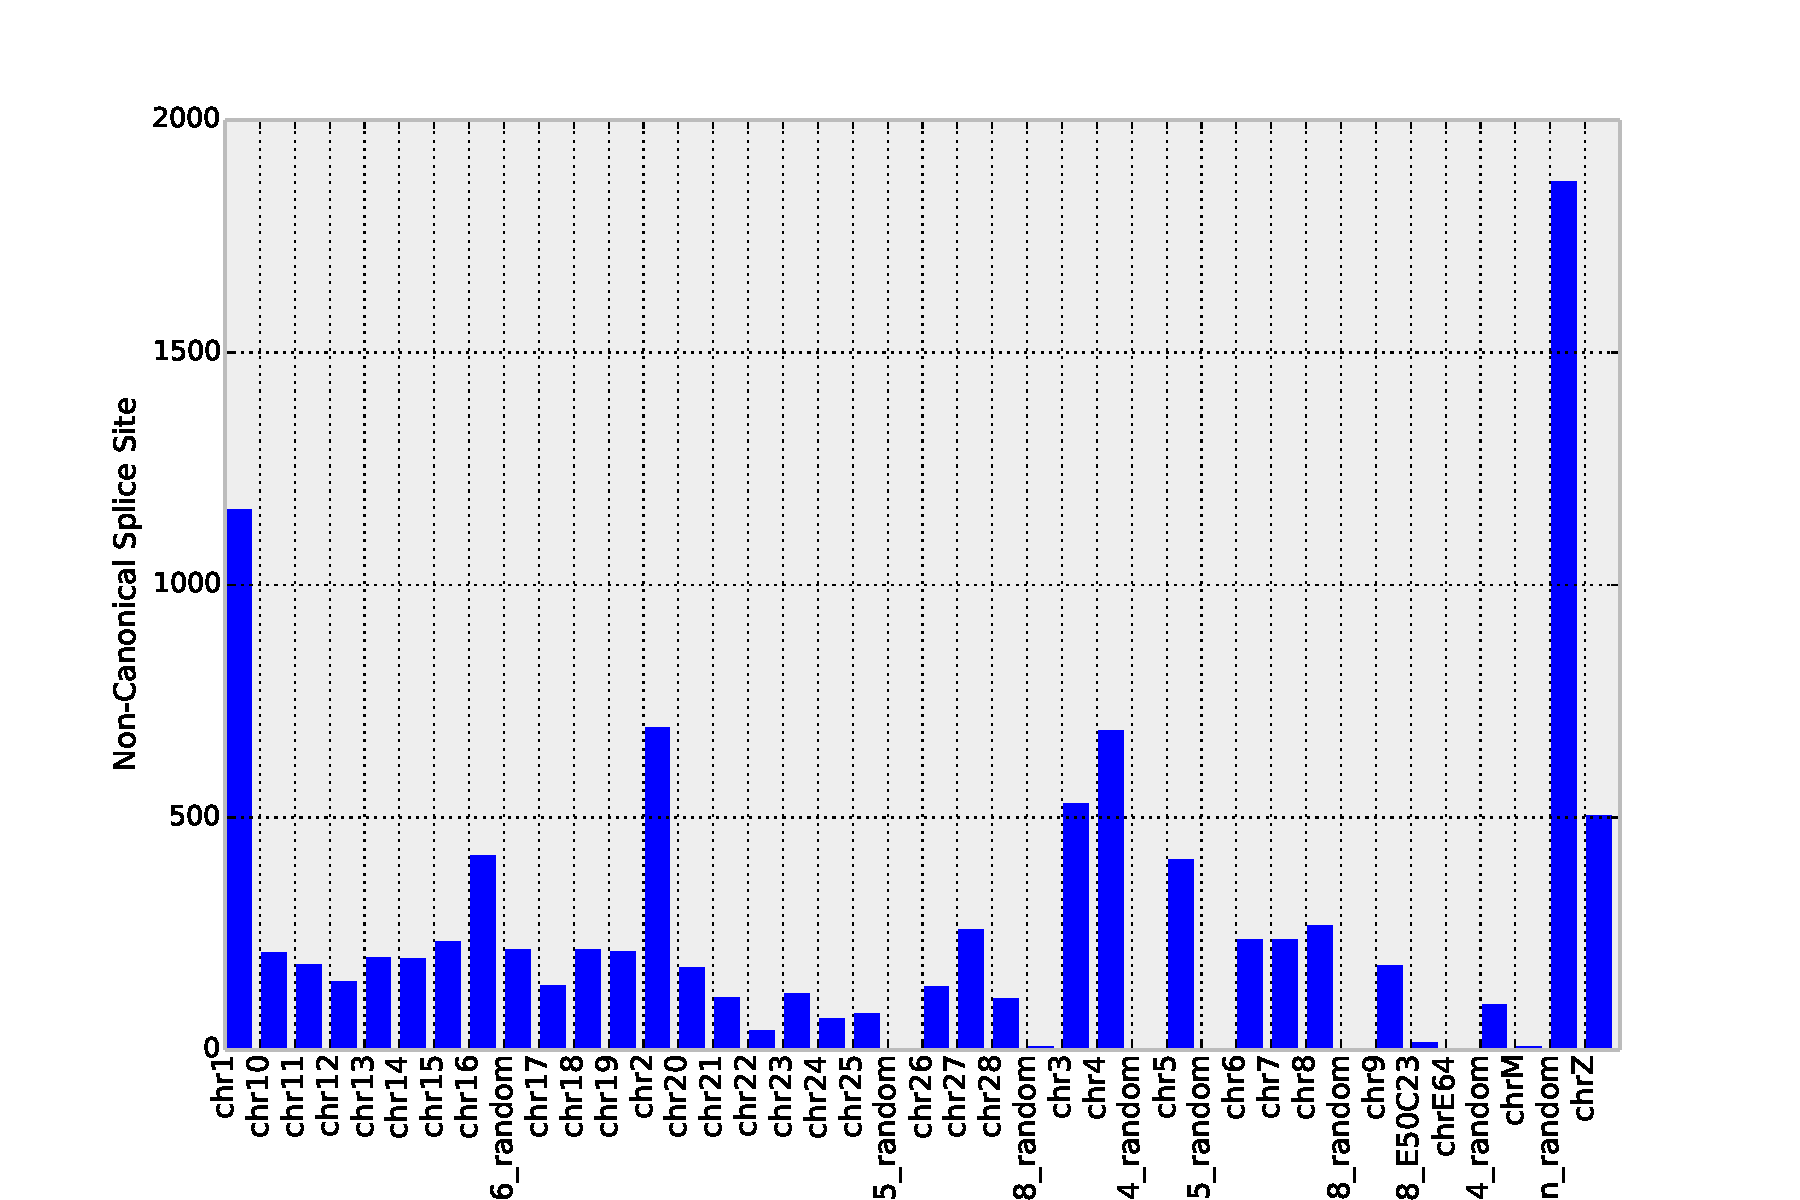
\includegraphics[width=6in]{noncanonical.pdf}
\end{center}
\caption{
{\bf Distribution of non-canonical splice sites.} A majority of non-canonical
splice sites are found in chrUn\_random, which may contain many misassemblies.}
\label{Figure_label}
\end{figure}

\begin{figure}[!ht]
\begin{center}
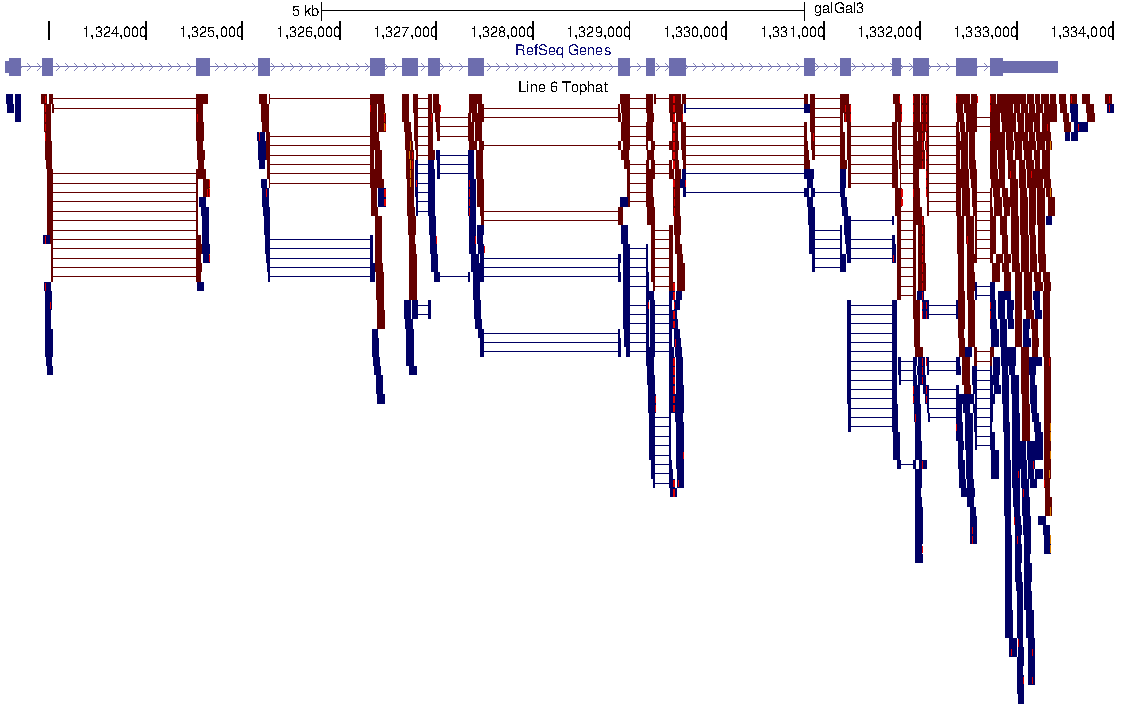
\includegraphics[width=6in]{read_bias.pdf}
\end{center}
\caption{
{\bf Read bias in RNA-Seq data.} In our datasets, the number of reads
mapped to reference genome gradually decreases toward the $5'$ end
of a transcript.
}
\label{Figure_label}
\end{figure}

\begin{figure}[!ht]
\begin{center}
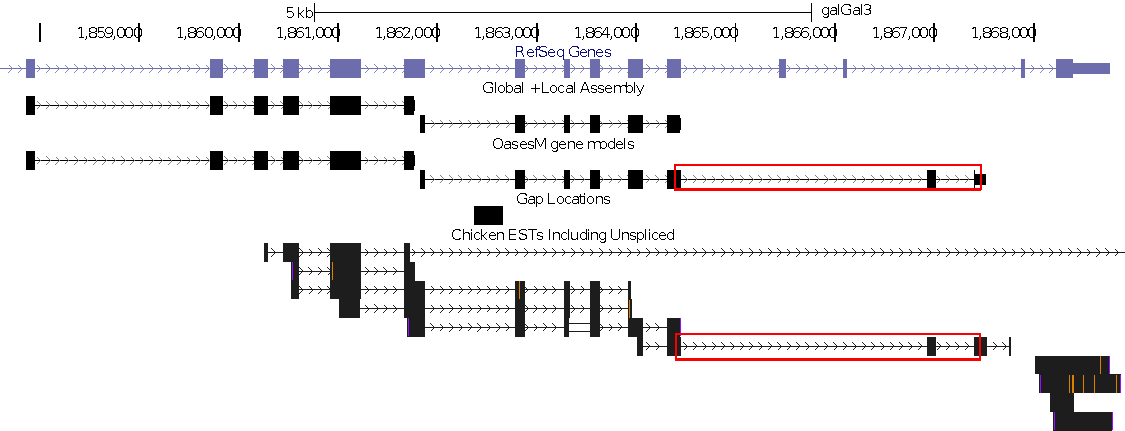
\includegraphics[width=6in]{uniq_junc_oasesM.pdf}
\end{center}
\caption{
{\bf Unique junction in OasesM transcripts.}
}
\label{uniq_junc_oasesM}
\end{figure}

\begin{figure}[!ht]
\begin{center}
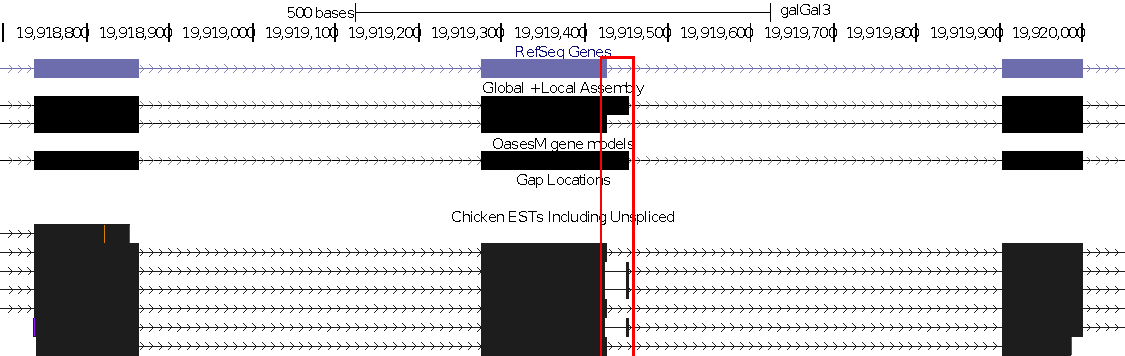
\includegraphics[width=6in]{uniq_junc_unmerged.pdf}
\end{center}
\caption{
{\bf Unique junction in unmerged transcripts.}
}
\label{uniq_junc_unmerged}
\end{figure}

\section*{Tables}
\begin{table}[!ht]
\caption{
\bf{Number of reads mapped to splice junctions}}
\begin{tabular}{cccccc}
\hline
Dataset & Model & Total & 0 reads& $\le3$ reads & $>3$ reads \\ 
\hline
Chicken & Assembly & 100,411 & 95 (0.09\%) & 448 (0.45\%) & 99,868 (99.46\%) \\
Chicken & Cufflink & 109,646 & 0 (0.0\%) & 1518 (1.38\%) & 108,128 (98.61\%) \\
Chicken & Assembly + Cufflink & 114,334 & 96 (0.08\%) & 1,597 (1.39\%) & 112,737 (98.60\%) \\
Mouse & Gimme & 111,795 & 536 (0.48\%) & 3,130 (2.78\%) & 108,129 (96.72\%) \\
Mouse & Cufflink & 88,476 & 130 (0.15\%) & 2,446 (2.76\%) & 85,900 (97.09\%) \\
\hline
%table information
\end{tabular}
%\begin{flushleft}\footnotesize \textit{}
%\end{flushleft}
\label{junction_read}

\end{table}

\begin{table}[!ht]
\caption{
\bf{Number of alignments of single-end reads to gene models by Bowtie}}
\begin{tabular}{cccc}
\hline
Model & Total* & Mapped** & Unmapped \\ 
\hline
Assembly & 199,572,442 & 183,832,752 (92.11\%) & 15,739,690 (7.88\%) \\
Cufflinks & 158,225,303 & 143,349,805 (90.60\%)& 14,875,498 (9.40\%) \\
Cufflinks + Gimme & 229,460,666 & 215,240,204 (93.80\%)& 14,220,462 (6.70\%) \\
\hline
%table information
\end{tabular}
\begin{flushleft}\footnotesize \textit{* Four datasets combined.\\
** $\le20$ alignments/read.}
\end{flushleft}
\label{junction_read}
\end{table}

\begin{table}[!ht]
\caption{
\bf{Number of single-end reads mapped to reference genome by Tophat}}
\begin{tabular}{cccc}
\hline
Dataset & Total & Mapped & Unmapped \\ 
\hline
Line 6 uninfected & 24,493,741 & 22,177,667 (90.54\%)& 2,316,074 (9.46\%) \\
Line 6 infected & 24,049,700 & 20,662,870 (85.92\%)& 3,386,830 (14.08\%) \\
Line 7 uninfected & 24,769,053 & 21,636,382 (87.35\%)& 3,132,671 (12.65\%) \\
Line 7 infected & 26,257,834 & 23,554,917 (89.71\%)& 2,702,914 (10.29\%) \\
\hline
%table information
\end{tabular}
%\begin{flushleft}\footnotesize \textit{*Minumum set}
%\end{flushleft}
\label{junction_read}
\end{table}

\begin{table}[!ht]
\caption{
\bf{Number of unique regions incorporated in gene models}}
\begin{tabular}{ccccc}
\hline
Dataset & \multicolumn{2}{c}{Unique Region} & \multicolumn{2}{c}{Incorporated*}\\
 & Global & Local & Global & Local\\
\hline
Line 6 uninfected & 12,037 & 1,716 & 3,088 (25.65\%) & 1,173 (68.36\%) \\
Line 6 infected & 13,502 & 2,781 & 3,478 (25.76\%) & 2,038 (73.28\%) \\
Line 7 uninfected & 12,445 & 2,170 & 4,031 (32.39\%) & 1,481 (68.25\%) \\
Line 7 infected & 13,582 & 1,683 & 4,129 (30.40\%) & 1,480 (87.94\%) \\
\hline
%table information
\end{tabular}
\begin{flushleft}\footnotesize \textit{*Matched gene models (BLAT) with
minimum identity $=90\%$, minimum coverage $=90\%$.}
\end{flushleft}
\label{uniq_regions}
\end{table}

\begin{table}[!ht]
\caption{
\bf{Unique regions from global and local assembly}}
\begin{tabular}{ccccccc}
\hline
Dataset & \multicolumn{2}{c}{Unique Region*} & \multicolumn{2}{c}{Matched with mouse proteins} & \multicolumn{2}{c}{Incorporated in gene models**}\\
 & Global & Local & Global & Local & Glocal & Local\\
\hline
Line 6 uninfected & 2,132 & 104 & 1,322 (62.01\%) & 39 (37.50\%) & 118 (5.53\%) & 103 (99.04\%) \\
Line 6 infected & 2,499 & 104 & 1,514 (60.58\%)& 40 (38.46\%) & 118 (4.72\%) & 95 (91.35\%) \\
Line 7 uninfected & 2,633 & 136 & 1,560 (59.25\%) & 52 (38.24\%) & 139 (5.28\%) & 124 (91.18\%) \\
Line 7 infected & 2,409 & 152 & 1,390 (57.70\%)& 50 (32.89\%) & 145 (6.02\%) & 150 (98.68\%) \\
\hline
%table information
\end{tabular}
%\begin{flushleft}Table Caption
%\end{flushleft}
\label{unique_sequences_matched_mouse}
\begin{flushleft}\footnotesize \textit{*Sequence length $\ge300$ bp.\\
**Matched gene models (BLAT) with minimum identity $=90\%$,
minimum coverage $=90\%$.}
\end{flushleft}
\label{uniq_regions}
\end{table}

\begin{table}[!ht]
\caption{
\bf{Unique sequences from global and local assembly}}
\begin{tabular}{ccccc}
\hline
Dataset & \multicolumn{2}{c}{Total Sequence (Kbp)} & \multicolumn{2}{c}{Unique Sequence (Kbp)}\\
 & Global & Local & Global & Local\\
\hline
Line 6 uninfected & 77,454.44 & 43,173.57 & 2,712.79 (3.5\%) & 327.00 (0.76\%)\\
Line 6 infected & 86,622.62 & 44,576.98 & 3,207.87 (3.7\%) & 446.06 (1.00\%)\\
Line 7 uninfected & 76,566.72 & 40,073.64 & 3,175.48 (4.15\%) & 399.29 (1.00\%)\\
Line 7 infected & 74,957.62 & 41,226.79 & 3,213.41 (4.29\%) & 346.99 (0.84\%)\\
\hline
%table information
\end{tabular}
%\begin{flushleft}Table Caption
%\end{flushleft}
\label{unique_sequences}
\end{table}

\begin{table}[!ht]
\caption{
\bf{Unique sequence from global and local assembly}}
\begin{tabular}{ccccc}
\hline
Dataset & \multicolumn{2}{c}{Unique Sequence (Kbp)} & \multicolumn{2}{c}{Matched with mouse proteins (Kbp)}\\
 & Global & Local & Global & Local\\
\hline
Line 6 uninfected & 1,169.24 & 102.92 & 226.5 (19.38\%) & 10.90 (10.50\%)\\
Line 6 infected & 1,486.22 & 68.05 & 273.86 (18.43\%)& 7.27 (10.68\%)\\
Line 7 uninfected & 1,647.23 & 113.81 & 306.70 (18.62\%) & 12.04 (10.58\%)\\
Line 7 infected & 1,505.81 & 136.68 & 260.62 (17.31\%)& 12.35 (9.04\%)\\
\hline
%table information
\end{tabular}
%\begin{flushleft}Table Caption
%\end{flushleft}
\label{unique_sequences_matched_mouse}
\end{table}

\end{document}
